\documentclass[10pt,a4paper]{article}
\usepackage{geometry}
 \geometry{
 a4paper,
 total={170mm,257mm},
 left=20mm,
 top=20mm,
 }


\usepackage[utf8]{inputenc}
\usepackage[spanish]{babel}
\usepackage{graphicx}
\usepackage{wrapfig}
\usepackage{amssymb, amsmath}
\usepackage{tikz}
\usepackage{enumitem}

\title{Calculo Eléctrico Líneas Subterráneas}
\author{MakerGarage}
\date{Abril 2021}


\setlength{\parindent}{0cm}


\renewcommand{\thesubsection}{\Roman{subsection}}
\renewcommand{\thesubsubsection}{\alph{subsubsection})}

\begin{document}

\maketitle
\newpage
\tableofcontents
\newpage

\section{Longitud crítica}
$$
L_{c}=\frac{I_{z} \cdot \sqrt{3} \cdot 10^{3}}{U_{n} \cdot \omega \cdot C}(\mathrm{~km})
$$
Donde:
\begin{itemize}
    \item $I_z$ es la intensidad máxima admisible del cable [A]
    \item $U_n$ es la tensión de línea en [kV]
    \item $C$ es la capacidad de la línea en [$\frac{\mu F}{km}$]
\end{itemize}

\section{Calcular la máxima potencia activa que pueden transportar una línea en función de su longitud, para una carga resistiva conectada en su extremo, teniendo en cuenta la carga capacitiva del cable}
$$
S_{G}=\sqrt{3} \cdot U_{n} \cdot I_{z} \cdot 10^{-6} [MVA]
$$
$$
P_{L}=\sqrt{S_{G}^{2} \cdot 10^6 -\left(\omega \cdot C \cdot L \cdot U_{n}^{2}\right)^{2}} \cdot 10^{-6} [MW]
$$
Donde:
\begin{itemize}
    \item $U_n$ es la tensión de línea en [V]
    \item $I_z$ es la intensidad máxima admisible del cable [A]
    \item $L$ es la longitud de la línea en [km]
    \item $C$ es la capacidad de la línea en [$\frac{F}{km}$]
\end{itemize}

\section{Densidad de corriente máxima admisible}
$$
\frac{I_{c c}}{S}=\frac{K}{\sqrt{t_{c c}}} \sqrt{\frac{\ln \left(\frac{\theta_{c c}+\beta}{\theta_{i}+\beta}\right)}{\ln \left(\frac{\theta_{c c}+\beta}{\theta_{s}+\beta}\right)}} [\frac{A}{mm^2}]
$$
Donde:
\begin{itemize}
    \item $K$ Tabla 25(cobre) 26(aluminio) de la pg70
    \item $\sqrt{t_{c c}}$ es el tiempo de cortocircuito en [s]
    \item $\beta$ es 235 (cobre) 228 (aluminio)
    \item $\theta_{s}$ es la temperatura máxima admisible del conductor pg58
    \item $\theta_{cc}$ es la temperatura máxima admisible del conductor en cortocircuito pg58
    \item $\theta_{i}$ es la temperatura inicial del conductor (es dato que nos da el enunciado)
\end{itemize}
\newpage
\section{La sección mínima del conductor según criterio de intensidad máxima en régimen 
permanente}
\subsection{Elección de la tensión nominal}
Para seleccionar la tensión nominal debemos de seleccionar la categoría (A-B-C [pg46]) en función del tiempo de desconexión, una vez tenemos la categoría miramos en la tabla 2 [pg47] y seleccionamos el valor de $U_o$.

\subsection{Cálculo de la sección del cable por intensidad máxima admisible}
$$
I_{real}=\frac{P_{n}}{\sqrt{3} \cdot U_{n} \cdot \cos \varphi} [A]
$$
ó
$$
I_{real}=\frac{S}{\sqrt{3} \cdot U_{n}} [A]
$$
Donde:
\begin{itemize}
    \item $P_n$ Potencia a transportar [kW]
    \item $U_n$ Tensión [kV]
    \item $\cos \varphi$ factor de potencia
    \item $S$ Potencia a transportar [kVA]
\end{itemize}

Procedemos a calcular la $I_{max}$ del conductor en las condiciones que nos indiquen
La $I_{max}$ se coge de la tabla 6 [pg59] en caso de ser conductor directamente enterrado, en caso de ir enterrado bajo tubo debemos mirar la tabla 12 [pg62].
\\

A este valor de $I_{max}$ debemos de aplicarle los factores de corrección correspondientes.
\\

Verificamos que:
$$
I_{real} < I_{max}
$$
\newpage
\section{La sección mínima del conductor que soporta térmicamente la intensidad de 
cortocircuito}
Si el dato del problema es la potencia de cortocircuito en MVA, la intensidad de cortocircuito 
vendrá dada por:
$$
I_{real\, cc}=\frac{S_{c c}}{\sqrt{3} \cdot U_{n}} [kA]
$$
Donde:
\begin{itemize}
    \item $S_{cc}$ Potencia de cortocircuito [MVA]
    \item $U_n$ Tensión [kV]
\end{itemize}

Ahora podemos o bien fijar $Icc = I_{real\, cc}$ y calcular el tiempo de desconexión 
$$
t_{c c}=\left[\frac{K \cdot S}{I_{real\,cc}\cdot 10^3} \sqrt{\frac{\ln \left(\frac{\theta_{c c}+\beta}{\theta_{i}+\beta}\right)}{\ln \left(\frac{\theta_{c c}+\beta}{\theta_{s}+\beta}\right)}}\right]^{2} [s]
$$

Comprobamos que:
$$t_{cc} > \text{tiempo de desconexión que nos dan}$$

O podemos fijar el $tcc = \text{tiempo de desconexión}$ y calcular la intensidad de cortocircuito que soporta la línea en estas condiciones
$$
I_{c c}=\frac{K \cdot S}{\sqrt{t_{c c}}} \sqrt{\frac{\ln \left(\frac{\theta_{c c}+\beta}{\theta_{i}+\beta}\right)}{\ln \left(\frac{\theta_{c c}+\beta}{\theta_{s}+\beta}\right)}} \cdot 10^{-3} [kA]
$$

Comprobamos que:
$$
I_{cc} > {I_{\text{real cc}}}
$$

Donde:
\begin{itemize}
    \item $K$ Tabla 25(cobre) 26(aluminio) de la pg70
    \item $S$ Sección del conductor [$mm^2$]
    \item $\sqrt{t_{c c}}$ es el tiempo de cortocircuito en [s]
    \item $\beta$ es 235 (cobre) 228 (aluminio)
    \item $\theta_{s}$ es la temperatura máxima admisible del conductor pg58
    \item $\theta_{cc}$ es la temperatura máxima admisible del conductor en cortocircuito pg58
    \item $\theta_{i}$ es la temperatura inicial del conductor (se calcula justo ahora despúes)
    
\end{itemize}

$$
\theta_{i}=\theta_{a}+\left(\theta_{s}-\theta_{a}\right) \cdot\left(\frac{I_{i}}{I_{z}}\right)^{2}
$$
Donde:
\begin{itemize}
    \item $\theta_{i}$ es la temperatura inicial del conductor
    \item $\theta_{a}$ es la temperatura media del terreno (dato que nos dan)
    \item $\theta_{s}$ es la temperatura máxima admisible del conductor pg58
    \item $I_i$ es $Ireal$ calculado con la fórmula del punto 4 $I_{real}=\frac{P_{n}}{\sqrt{3} \cdot U_{n} \cdot \cos \varphi} [A]$
    \item $I_z$ es $I_{max}$ con los factores de corrección aplicados (punto 4).
\end{itemize}

\newpage
\section{Máxima caída de tensión admisible por el conductor}
$$
\Delta U=\sqrt{3} \cdot I \cdot L \cdot(R \cdot \cos \varphi+X \cdot \operatorname{sen} \varphi) [V]
$$

$$
\frac{\Delta U}{U_n} \cdot 100 < 5\% (\text{según el enunciado})
$$
Donde:
\begin{itemize}
    \item $I$ es $I_{real}$
    \item $L$ es la longitud de la linea [km]
    \item $R$ es la resistencia en $\frac{\Omega}{km}$
    \item $X$ es la impedancia en $\frac{\Omega}{km}$
    \item $U_n$ Tensión [V]
\end{itemize}
Para obtener el valor de R podemos recurrir a los datos que da el fabricante para la máxima temperatura de servicio en régimen permanente, 90 ºC o bien calcularlo a partir de la resistividad del aluminio a 20 ºC, considerando la temperatura real de servicio en función de la intensidad que circula por el conductor y teniendo en cuenta tanto el efecto pelicular como el efecto proximidad.

\section{Elementos de un conductor}
\begin{center}
    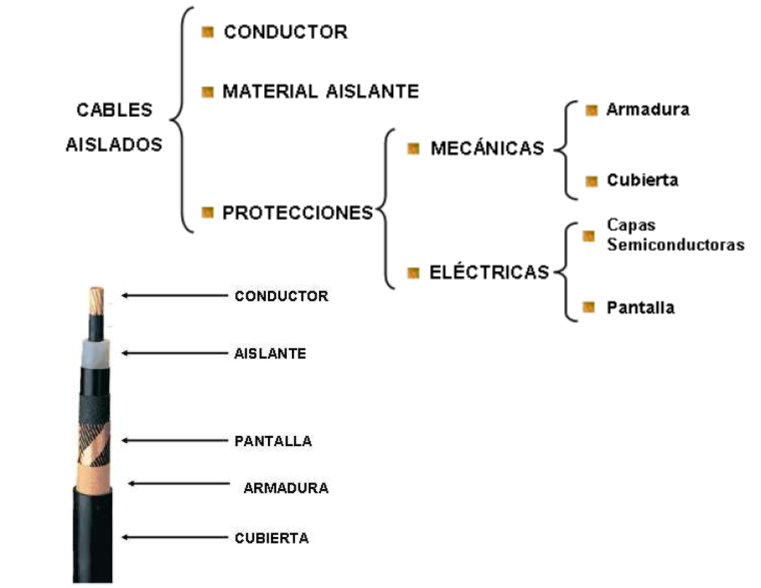
\includegraphics[scale = 0.8]{Elementos.png}
\end{center}
\section{Conductor enterrado}
\begin{center}
    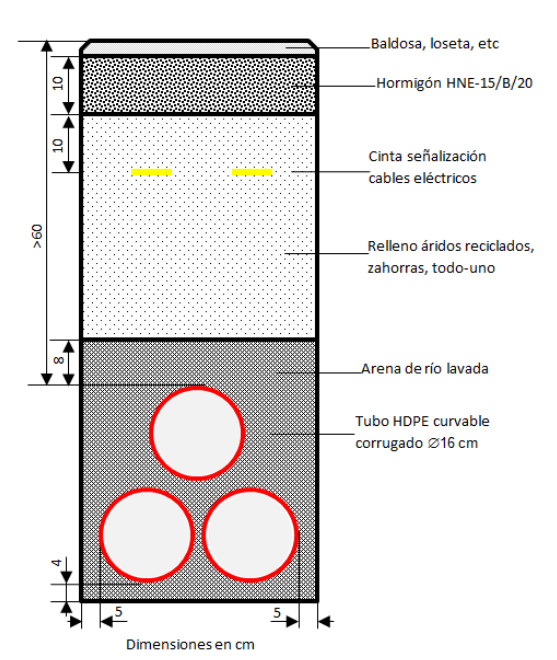
\includegraphics[scale = 0.6]{Captura de pantalla 2021-05-09 110303.png}
\end{center}

\section{Puesta a tierra de las pantallas}
Durante el funcionamiento de un circuito se inducen en las pantallas de los
conductores unas tensiones, y dependiendo del sistema de conexión de puesta a
tierra de las pantallas se pueden dar dos fenómenos distintos:
\begin{itemize}
    \item Aparecer corrientes inducidas que disminuyen la capacidad de transporte.
    \item Aparecer tensiones inducidas que pueden alcanzar valores peligrosos para la seguridad de personas o valores capaces de dañar los materiales de la instalación o reducir la vida útil de los mismos.
\end{itemize}


Las principales funciones del sistema de conexión de puesta a tierra serán:
\begin{itemize}
    \item  Eliminar o reducir corrientes de circulación por las pantallas debidas a un acoplamiento inductivo con la corriente que pasa por los cables, evitando así pérdidas de potencia activa.
    \item Reducir las tensiones inducidas entre las pantallas de los cables y tierra, tanto en régimen permanente como en cortocircuito. Las sobretensiones inducidas durante cortocircuitos pueden provocar averías en los cables, principalmente en los empalmes, terminales y en las cajas de conexiones que se utilizan para la transposición de pantallas, así como la perforación del aislamiento de la cubierta.
\end{itemize}

En las instalaciones de líneas subterráneas se utilizará uno de los
sistemas de puesta a tierra que se describen a continuación:
\begin{itemize}
    \item Sistema de conexión rígida a tierra.\begin{itemize}
        \item Sistema de puesta a tierra Solid Bonding (puesta a tierra en ambos
extremos).
    \end{itemize}
    \item Sistemas de conexión especial a tierra. \begin{itemize}
        \item Sistema de puesta a tierra Single Bonding (puesta a tierra en un solo extremo)
        \item Sistema de puesta a tierra Cross Bonding (con transposición de
pantallas)
    \end{itemize}
\end{itemize}
\subsection{Solid Bonding}
Con la utilización de este sistema de puesta a tierra no se disponen medidas
para evitar la circulación de corrientes por las pantallas en régimen
permanente. Estas corrientes inducidas por los conductores, originan calor,
con la consiguiente disminución de la capacidad de transporte.
\\

Este sistema de puesta a tierra de las pantallas se utilizará únicamente en
líneas subterráneas de muy corto recorrido y en los casos en que las
pérdidas de potencia pueda ser asumible (Media Tensión).
\begin{center}
    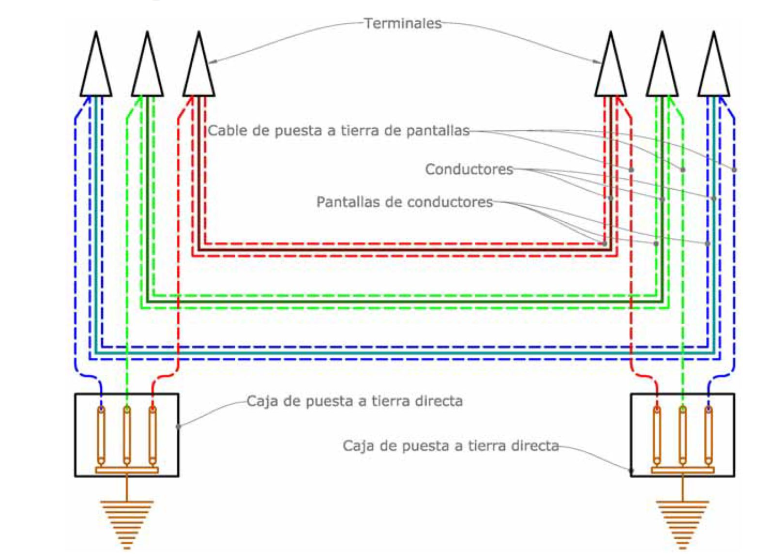
\includegraphics[scale = 0.6]{SolidBonding.png}
\end{center}
\newpage
\subsection{Single Bonding}
Este tipo de conexión se utilizará para cables de tension asignada igual o
superior a 26/45 kV en líneas de pequeña longitud, con uno o dos tramos
como máximo, en las que se requiere el aprovechamiento al máximo de la
intensidad admisible del conductor sin las limitaciones que provocan las
corrientes de pantalla.
Dentro de este sistema se pueden distinguir dos variantes del tipo de
conexión:
\begin{itemize}
    \item Conexión Single-Point que se utiliza en tramos cortos y sin empalmes
    \begin{center}
        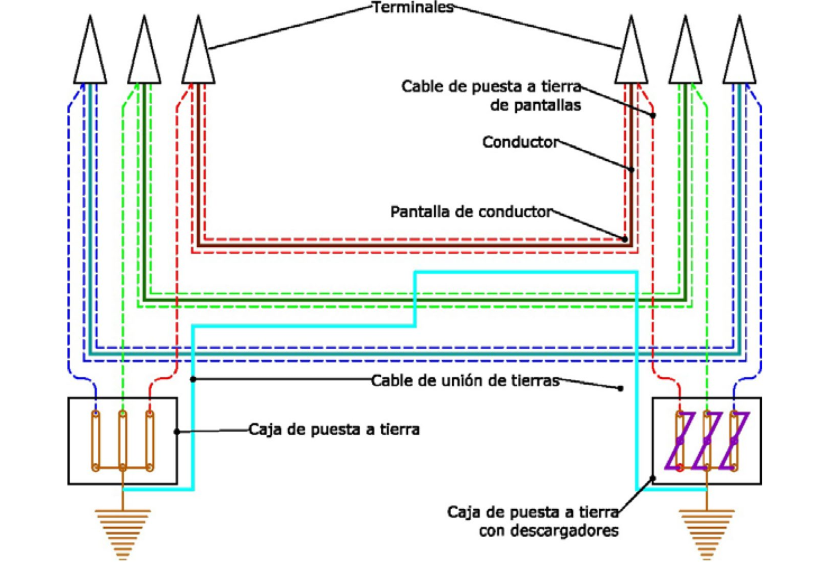
\includegraphics[scale = 0.6]{SinglePoint.png}
    \end{center}
    \item  Conexión Mid-Point, o Doble Single-Point, que se utiliza para tramos más largos en los que el tendido de los conductores se realiza en dos tramos, y con un empalme en el punto medio del trazado
    \begin{center}
        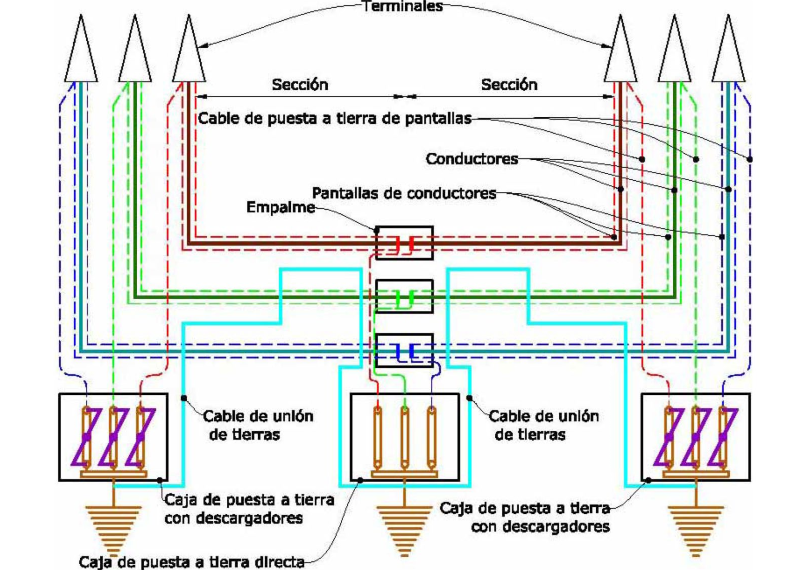
\includegraphics[scale = 0.6]{MidPoint.png}
    \end{center}
\end{itemize}

\newpage
\subsection{Cross Bonding}
Se utilizará este Sistema para cables de tension asignada igual o superior a 26/45 kV, en líneas en las que su longitud implique la realización de al menos 2 empalmes por conductor, y dónde se quiera eliminar las corrientes de pantalla.
\\
El sistema Cross-Bonding consiste en la distribución de las pantallas de cable en secciones elementales llamadas secciones menores, y cruzando las pantallas de tal manera que se neutralice la totalidad del voltaje inducido en 3 secciones consecutivas.
\\
Se interrumpirán las pantallas de cada conductor en los puntos de transposición para poder ejecutarla. Las tres secciones menores juntas forman una sección mayor. En un sistema de cruzamiento de pantallas, el tramo de línea a considerar se divide en 3 longitudes iguales (así el sistema quedará eléctricamente equilibrado), con las pantallas puestas a tierra en los dos extremos de la línea conectada en Cross-Bonding o en los dos extremos de cada sección mayor. De esta manera se induce una tensión entre la pantalla y tierra pero se eliminan las corrientes inducidas.
\begin{center}
        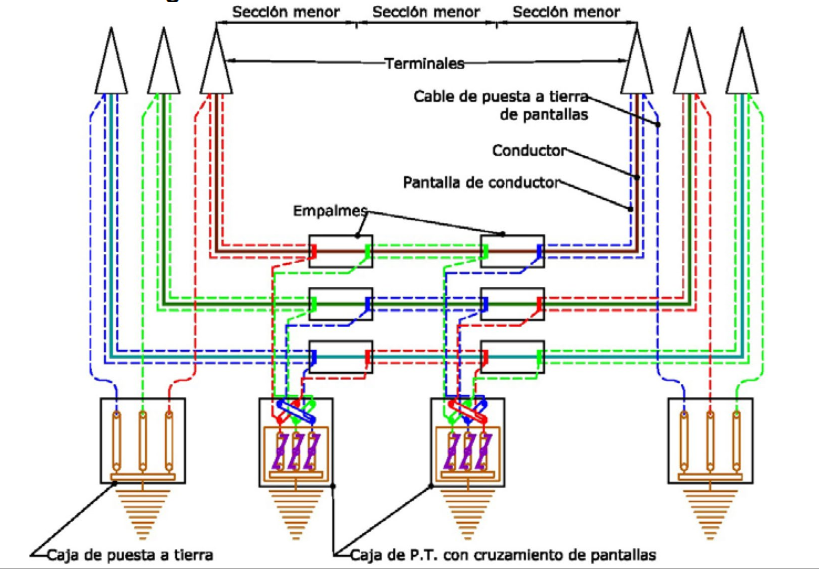
\includegraphics[scale = 0.6]{Cross.png}
    \end{center}


\end{document}
